\documentclass[dvipsnames,tikz]{standalone}
\usepackage{amsmath}
\usepackage{xcolor}
\usepackage{tikz}
\usepackage{cmbright}      % sansfont
\usetikzlibrary{calc}
\usetikzlibrary{decorations.pathreplacing,calligraphy,3d}

\tikzset{main/.style={draw=black, thick, circle, color=black}}

\begin{document}
	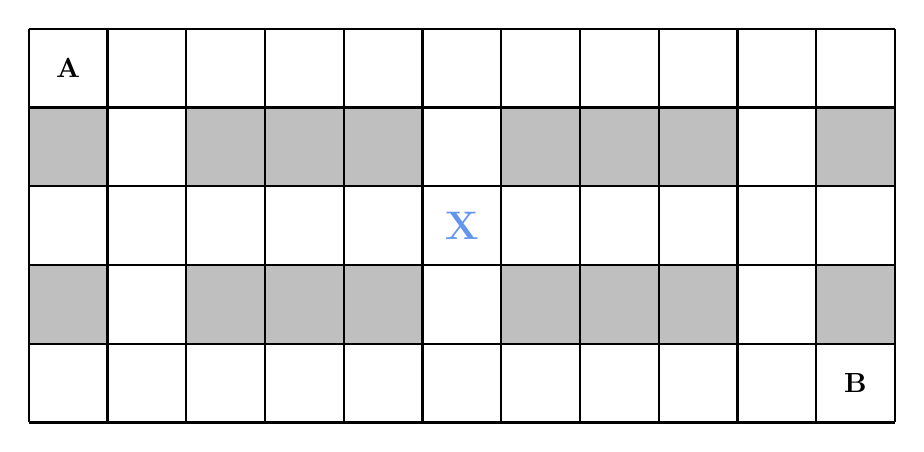
\begin{tikzpicture}[xscale=1]
		\fill[black!50, semitransparent] (0,3) rectangle ++(1,1) (0,1) rectangle ++(1,1) (2,1) rectangle ++(3,1) (2,3) rectangle ++(3,1) (6,3) rectangle ++(3,1) (6,1) rectangle ++(3,1) (10,3) rectangle ++(1,1) (10,1) rectangle ++(1,1) ;
		\draw[main] (0,0) grid (11,5);
		
		
		\draw[main] (0.5,4.5)node {\textbf A};
		\draw[main] (10.5,0.5)node {\textbf B};
		\draw[CornflowerBlue] (5.5,2.5)node {\Large \textbf X};
	\end{tikzpicture}

	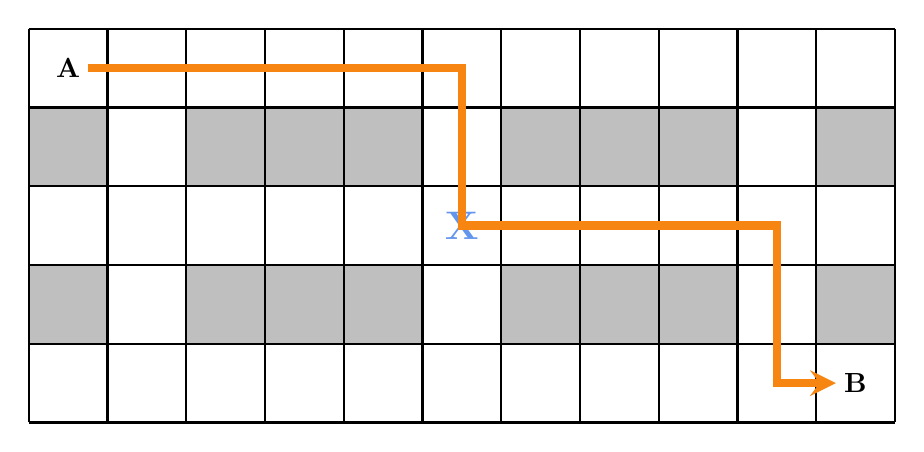
\begin{tikzpicture}[xscale=1]
		\fill[black!50, semitransparent] (0,3) rectangle ++(1,1) (0,1) rectangle ++(1,1) (2,1) rectangle ++(3,1) (2,3) rectangle ++(3,1) (6,3) rectangle ++(3,1) (6,1) rectangle ++(3,1) (10,3) rectangle ++(1,1) (10,1) rectangle ++(1,1) ;
		\draw[main] (0,0) grid (11,5);
		
		\draw[CornflowerBlue] (5.5,2.5)node {\Large \textbf X};
		
		\draw[line width=3pt, BurntOrange, -stealth] (0.5,4.5) ++(0.25,0) --++ (5-0.25,0) --++(0,-2) --++(4,0) --++(0,-2)--++(0.75,0);
		
		\draw[main] (0.5,4.5)node {\textbf A};
		\draw[main] (10.5,0.5)node {\textbf B};
	\end{tikzpicture}
	
	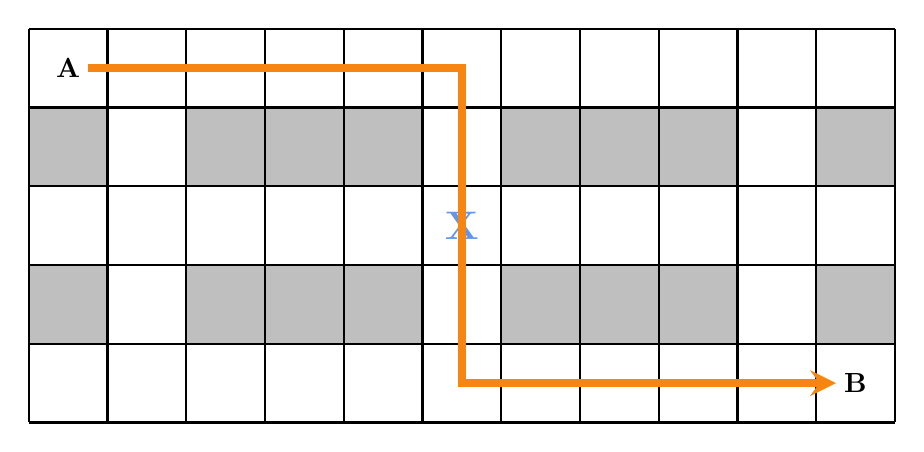
\begin{tikzpicture}[xscale=1]
		\fill[black!50, semitransparent] (0,3) rectangle ++(1,1) (0,1) rectangle ++(1,1) (2,1) rectangle ++(3,1) (2,3) rectangle ++(3,1) (6,3) rectangle ++(3,1) (6,1) rectangle ++(3,1) (10,3) rectangle ++(1,1) (10,1) rectangle ++(1,1) ;
		\draw[main] (0,0) grid (11,5);
		
		\draw[CornflowerBlue] (5.5,2.5)node {\Large \textbf X};
		
		\draw[line width=3pt, BurntOrange, -stealth] (0.5,4.5) ++(0.25,0) --++ (5-0.25,0) --++(0,-4) --++(4.75,0);
		
		\draw[main] (0.5,4.5)node {\textbf A};
		\draw[main] (10.5,0.5)node {\textbf B};
	\end{tikzpicture}

	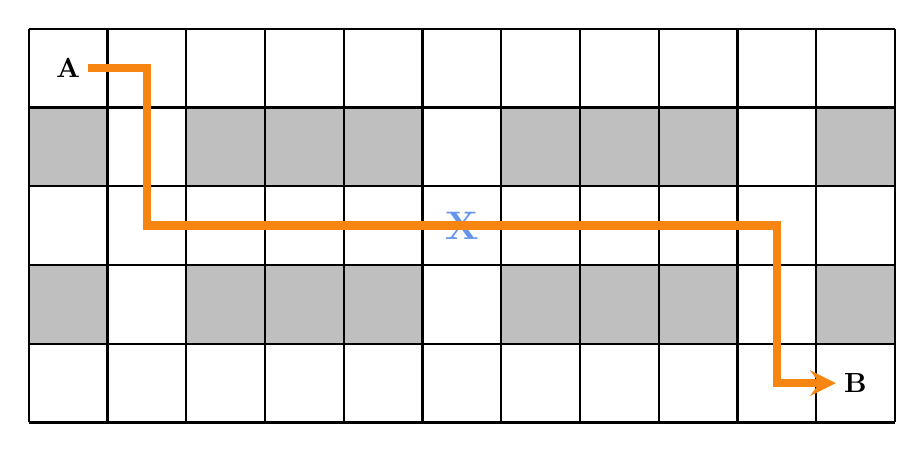
\begin{tikzpicture}[xscale=1]
		\fill[black!50, semitransparent] (0,3) rectangle ++(1,1) (0,1) rectangle ++(1,1) (2,1) rectangle ++(3,1) (2,3) rectangle ++(3,1) (6,3) rectangle ++(3,1) (6,1) rectangle ++(3,1) (10,3) rectangle ++(1,1) (10,1) rectangle ++(1,1) ;
		\draw[main] (0,0) grid (11,5);
		
		\draw[CornflowerBlue] (5.5,2.5)node {\Large \textbf X};
		
		\draw[line width=3pt, BurntOrange, -stealth] (0.5,4.5) ++(0.25,0) --++ (1-0.25,0) --++(0,-2) --++(8,0) --++(0,-2)--++(0.75,0);
		
		\draw[main] (0.5,4.5)node {\textbf A};
		\draw[main] (10.5,0.5)node {\textbf B};
	\end{tikzpicture}

	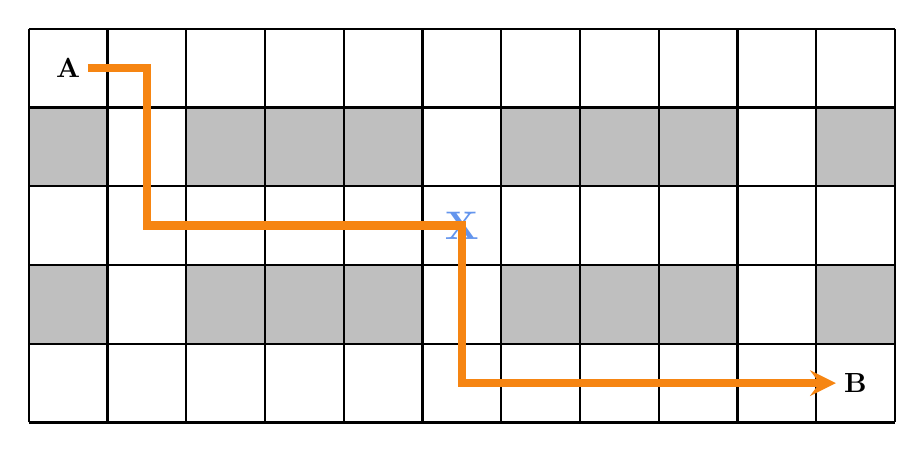
\begin{tikzpicture}[xscale=1]
		\fill[black!50, semitransparent] (0,3) rectangle ++(1,1) (0,1) rectangle ++(1,1) (2,1) rectangle ++(3,1) (2,3) rectangle ++(3,1) (6,3) rectangle ++(3,1) (6,1) rectangle ++(3,1) (10,3) rectangle ++(1,1) (10,1) rectangle ++(1,1) ;
		\draw[main] (0,0) grid (11,5);
		
		\draw[CornflowerBlue] (5.5,2.5)node {\Large \textbf X};
		
		\draw[line width=3pt, BurntOrange, -stealth] (0.5,4.5) ++(0.25,0) --++ (1-0.25,0) --++(0,-2) --++(4,0) --++(0,-2)--++(4.75,0);
		
		\draw[main] (0.5,4.5)node {\textbf A};
		\draw[main] (10.5,0.5)node {\textbf B};
	\end{tikzpicture}

\end{document}